\documentclass[12pt,a4paper,eval,english,firamath]{nsi}
\pagestyle{empty}
\begin{document}
\titre{Secret Santa}
\classe{Euro 1\ere}
\maketitle
\subsubsection*{From 00:00 to 00:42}
Explain what is Secret Santa.\\

\carreauxseyes{16.8}{4}

\subsubsection*{From 01:22 to 01:36}
What are the two fundamental things for a perfect Secret Santa ?\\

\carreauxseyes{16.8}{4}
\subsubsection*{From 01:44 to 02:03}
How does Hannah describe the "hat method" ?\\

\carreauxseyes{16.8}{5.6}

\subsubsection*{From 02:03 to 02:46}
What is the obvious problem with this method and what does the group have to do in this case ?\\

\carreauxseyes{16.8}{3.2}\\

Why is there also an anonymity violation if the person before the last one pulls his or her name ?\\

\carreauxseyes{16.8}{4}
\subsubsection*{From 02:46 to 10:59}
\picleft{0.25}{img/tree_santa3}{
    Despite of anonymity issues, let's see how  Secret Santa works with 3 persons.\\

    Complete this probability tree.\\

    When the method works, can we say is it completely random ?\\
    Justify your answer.}

\carreauxseyes{16.8}{4}
\subsubsection*{From 11:00 till the end}
Explain what's the right way to organize a Secret Santa.\\

\carreauxseyes{16.8}{8}
\subsection*{Bonus}

What's a derangement ?\\

\carreauxseyes{16.8}{4}\\

Complete the following tree for a "hat method" with 4 person.
\begin{center}
    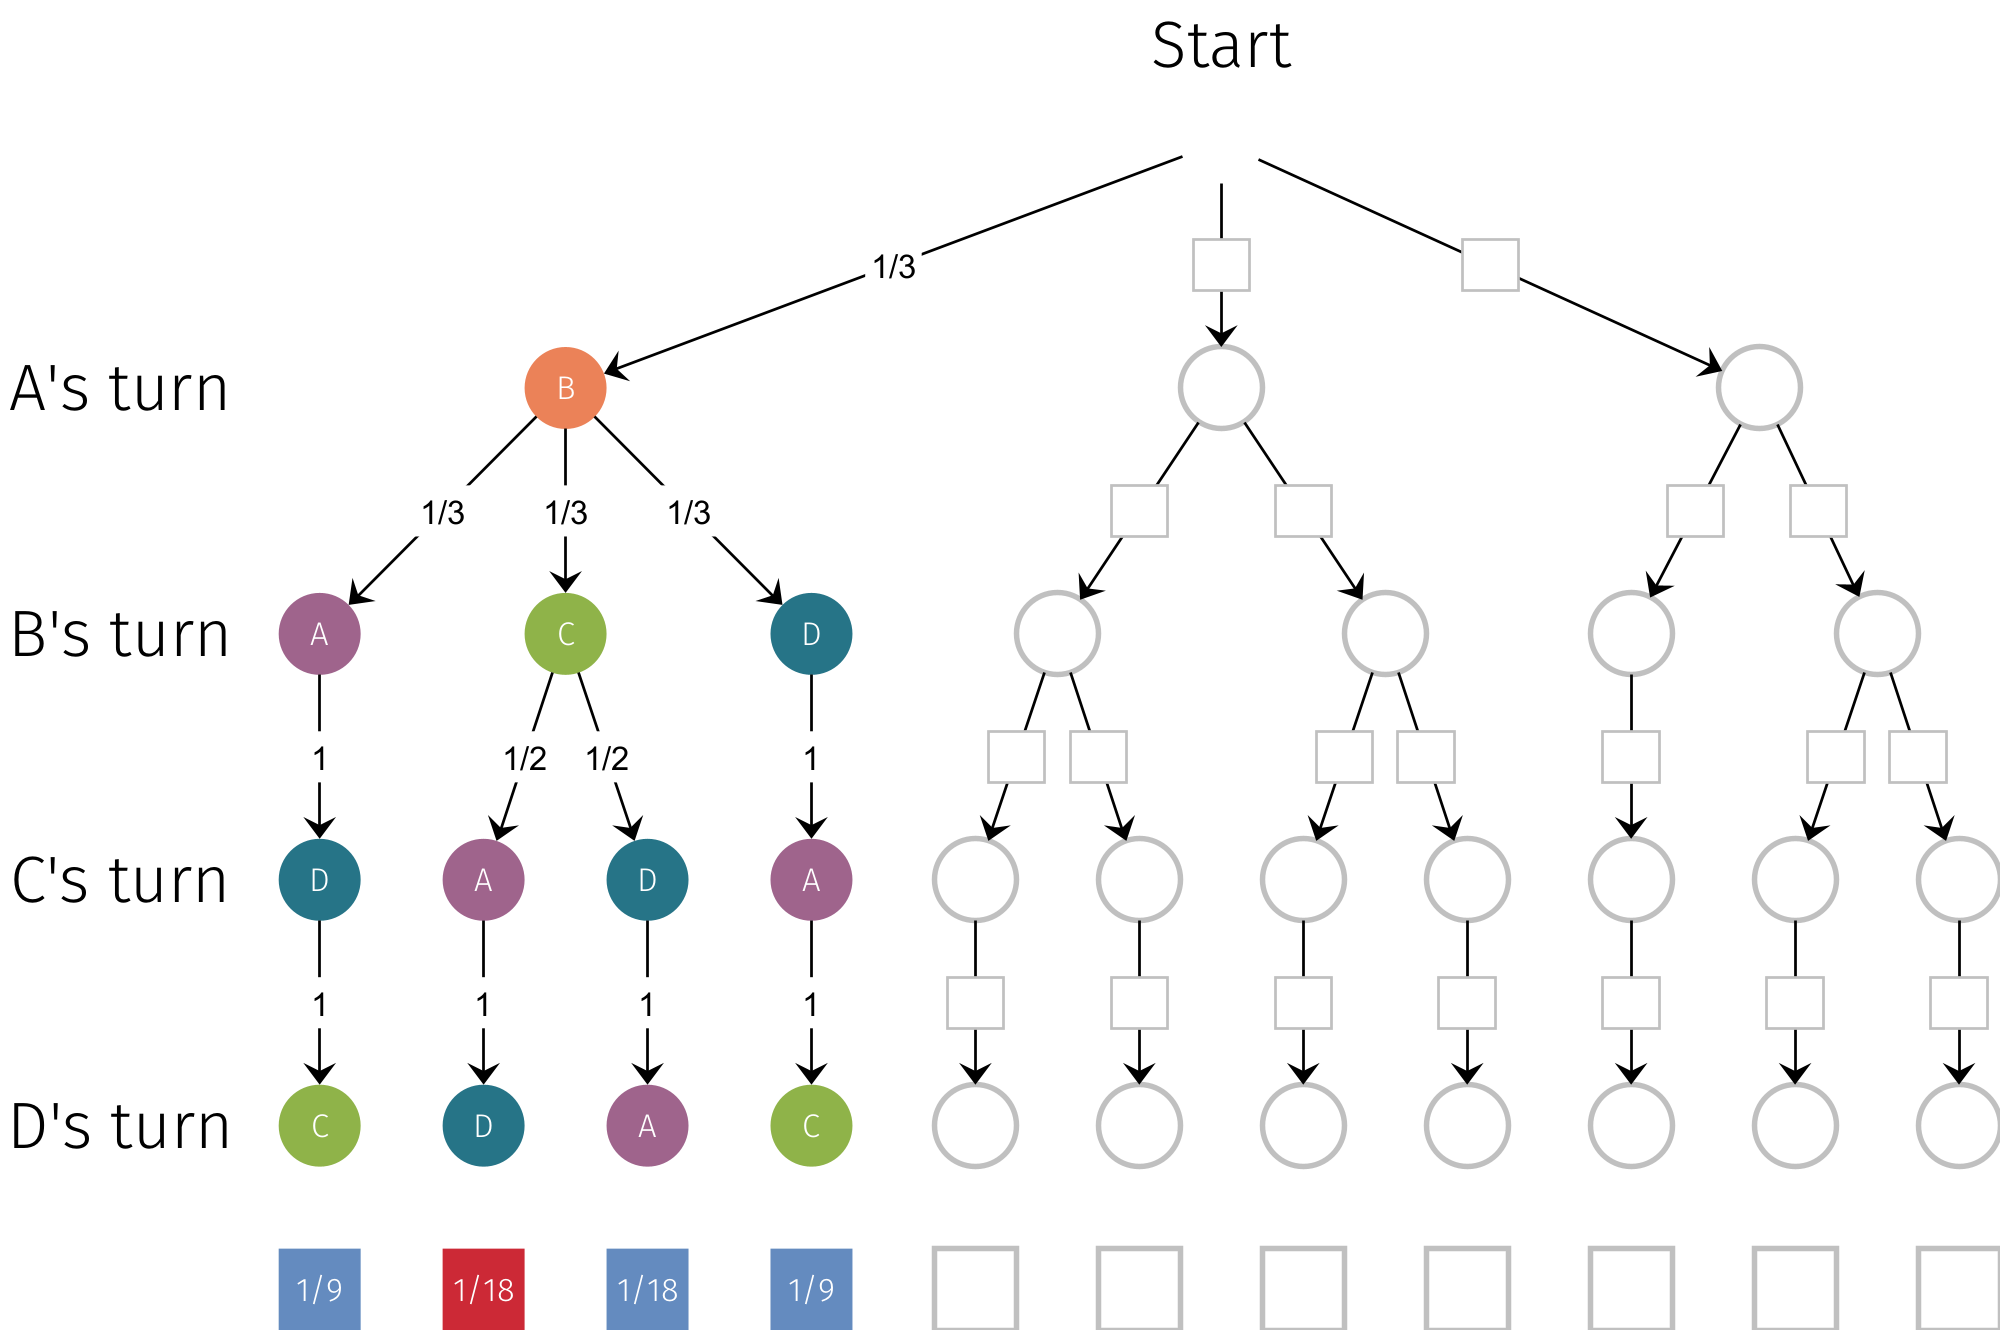
\includegraphics[width=16.8cm]{img/tree_santa4.png}
\end{center}
What's the probability of a failure ?\\

\carreauxseyes{16.8}{4}





\end{document}